\documentclass[../eva1_scion.tex]{subfiles}
\begin{document}
    \chapter{Results}
    \section{Isolation Domains}
    SCION borrows basic ideas from the Border Gateway Protocol (BGP) like the idea of an Autonomous System (AS) which, like in BGP, repesents the smalest organisational unit. However, SCION introduces an additonal organisational unit called the Isolation Domain (ISD). The structure of an indivual ISD is ilustrated in \ref{fig:isd}a. An ISD is comprised of multiple core ASes, form logical unit whos members share a common set of resources and mutualy trust each other. As their name states, ISDs are intended to be selfsuficient units, the internal state of which must not leak out into other ISDs. \cite{scion_2011} While an arbitrary AS can be a member of an arbitrary ISD, or even multiple ISDs, it is expected that ISDs will form along shared comercial interests, legal juristiction or other political borders. \cite{scion_2017}.

    \subsection{IDS structure}
    As shown in ilustration \ref{fig:isd}a the main structure of an IDS is an undirected graph formed by a set of core ASes in the ISD core, client ASes and biderectional links between individual ASes. ASes may be connected by multiple redundant links. Although a link always carries biderctional traffic, there is an implied top down hirarchy of providers and consumers between the tiers in the graph. As in BGP a pair of ASes may enter an peering agreement, which is ilustrated is a dashed line. Links are also called path segments.

    \subsection{AS and IDS Componants}
    In the following we will explore the componantes which are required to run an SCION AS and by extension a IDS since a single core AS is sufficient to form an IDS.

    SCION ASes look similar too their BGP cousins so fare as that they have internal routers and border routers and a set of routes through the AS. These ensure connectivity inside the AS and to neighbouring ASes. Border routers must be SCION enabled and must addhere to the common rules agreed upon inside de IDS, however each AS is free to choos its internal structure. In addition each AS needs at least a beacon server, a certificate server and a path server. Beacon servers are responbsible for path discovery and are required for beaconing process described in section \ref{ssec:beaconing}. Path server are repsonsible for caching and disimination of path information. They are involved in path resolution and assembly discussed in section \ref{ssec:path_assembly}. As SCION makes extensive us of certificates to validate paths and intities, certificate servers are deployed to cache and provide certificates in an AS.
    
    A core AS differs from other ASes in serveral important aspects. First of all Core ASes have border routers which are connected to cores ASes in neighbouring. The beacon servers in the core ASes also take part in inter IDS beaconing, thus their path servers also hold path information on how to reach neighbouring ASes. Further more the ISD core is responsible for maintaining the trust root configuration (TRC).
    \begin{figure}[h]
        \centering
        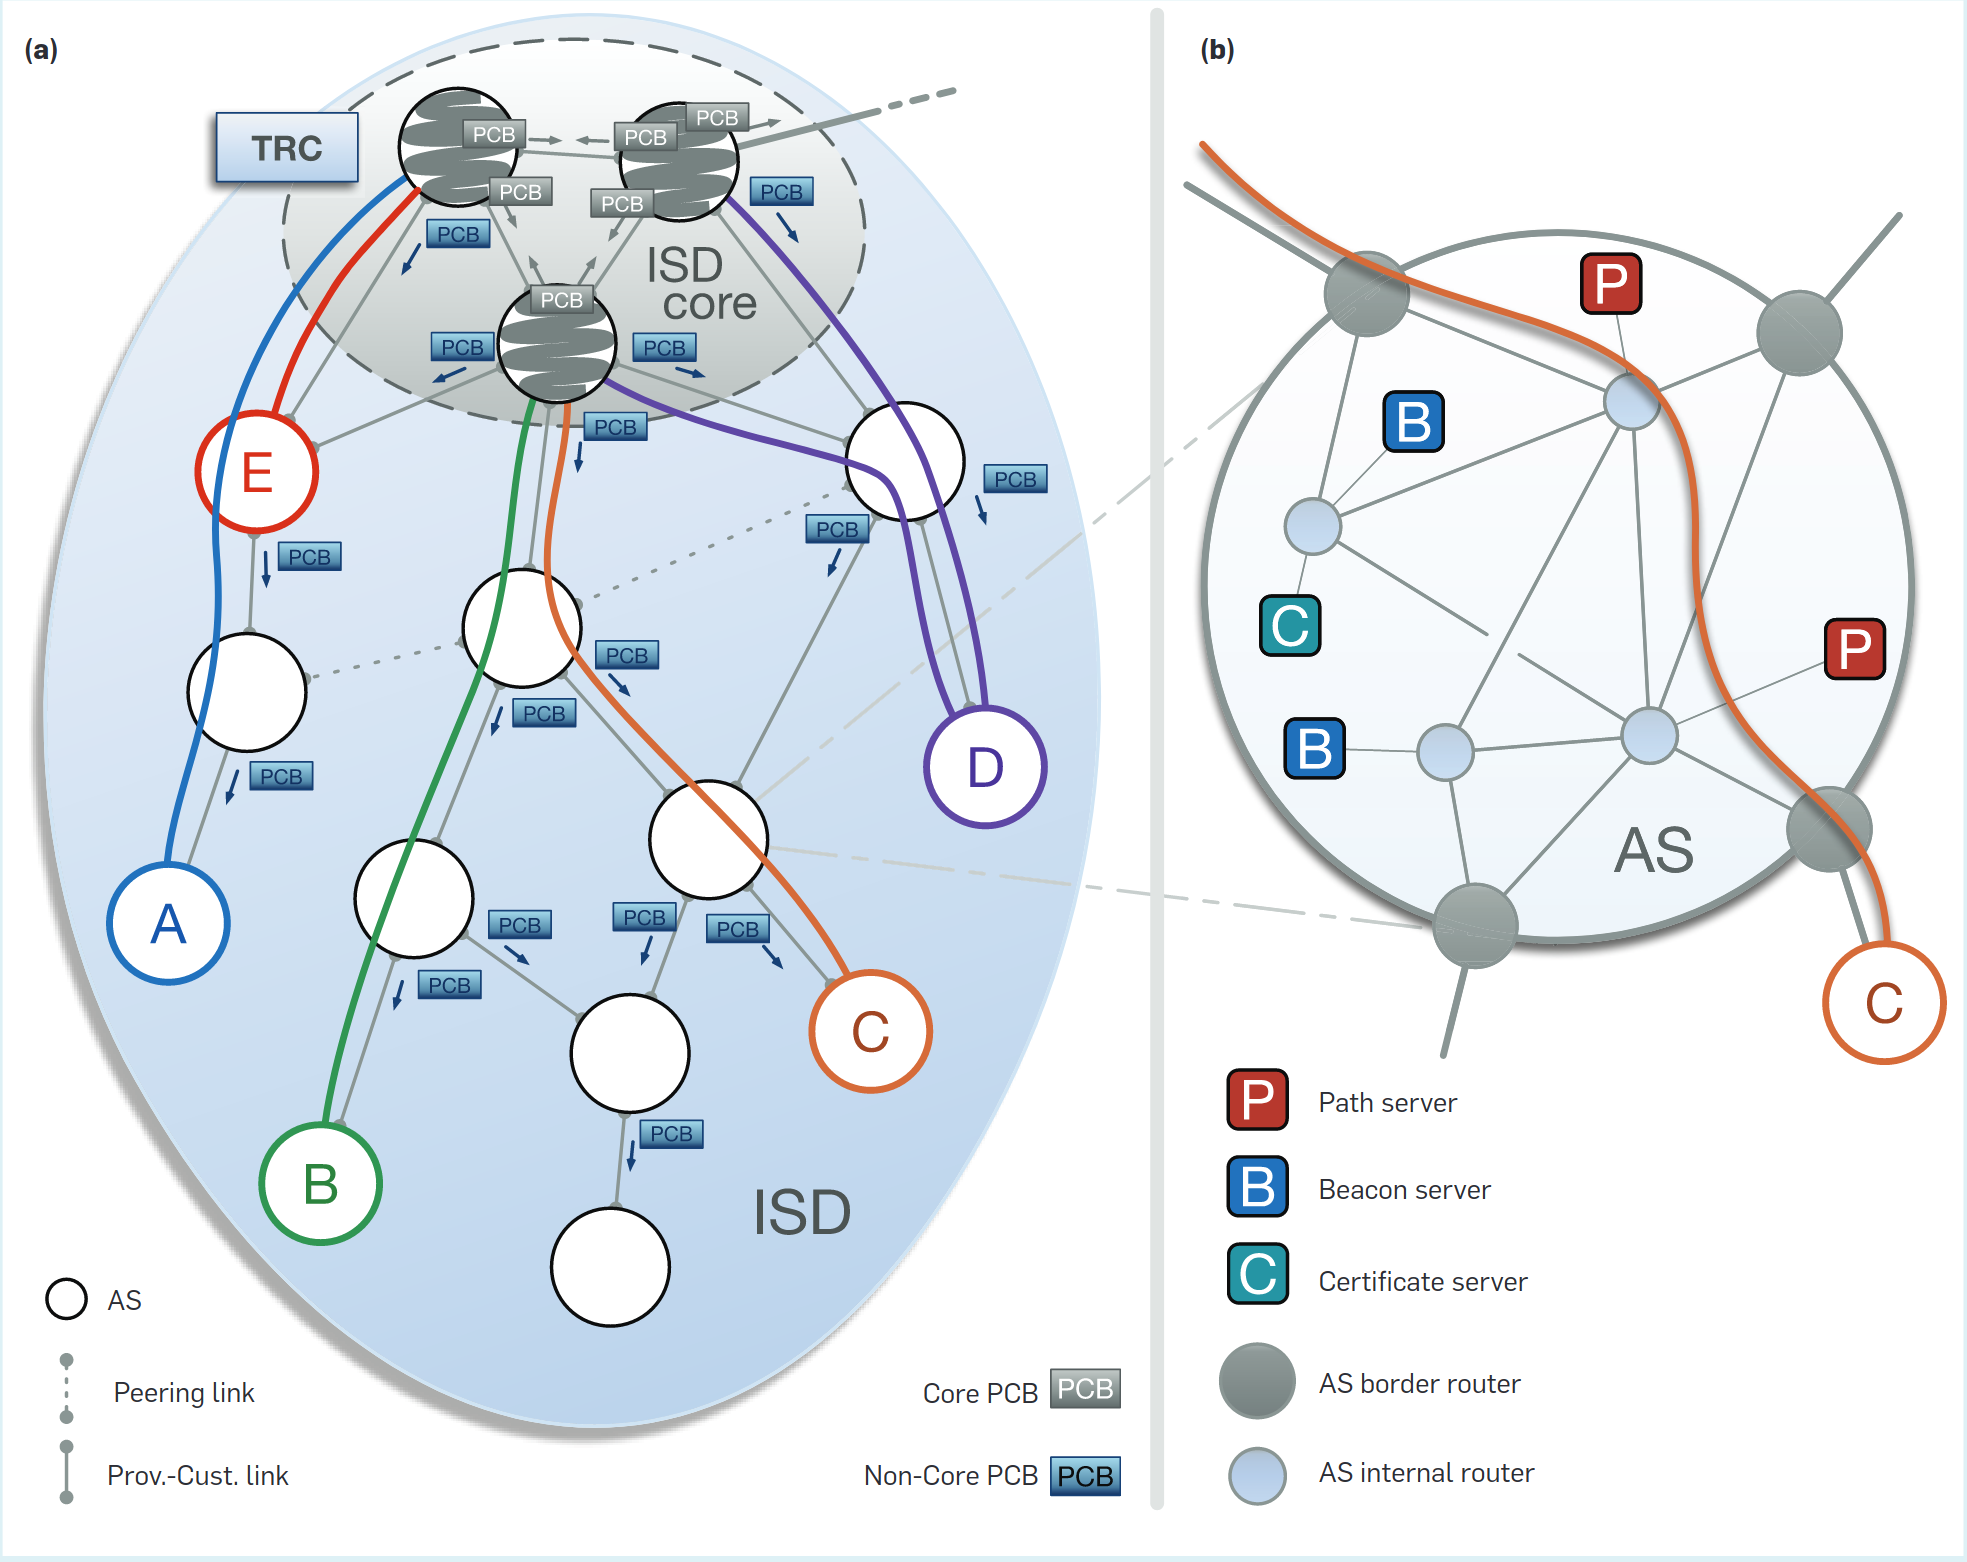
\includegraphics[width=0.8\linewidth]{scion_isd.png}
        \caption{Internal structure of an ISD. From \cite{scion_2017}}%
        \label{fig:isd}
    \end{figure}

    \section{Control Plane}
    \subsection{Path Discovery by Beaconing}\label{ssec:beaconing}
    \section{Data Plane}

    \subsection{Path Assembly} \label{ssec:path_assembly}
    \subsection{Data Forwading}
    
    \section{Trust Management}
    
    \section{SCION Adoption}


\end{document}
